\documentclass[12pt,a4paper]{article}

\usepackage[fleqn]{amsmath} % This package with the fleqn option aligns equations to the left
\setlength{\mathindent}{0pt} % Set indentation from the left margin

\usepackage{amssymb} % Required for math symbols
\usepackage{graphicx} % Required for inserting images
\usepackage{geometry}

\usepackage[backend=biber, style=authoryear, citestyle=authoryear]{biblatex}
\addbibresource{references.bib}

\geometry{a4paper, margin=1in}

{
\title{
    
\includegraphics[width=0.34\textwidth]{/Users/mlnick/documents/images/tsukuba-logo.png} \\
    \textbf{Principles of Software Engineering} \\
    \vspace{3mm}    
    Final Report
}

\author{Mamanchuk Mykola, SID.202420671}
\date{\today}
}

\usepackage{listings}
\usepackage{color}

\definecolor{codegreen}{rgb}{0,0.6,0}
\definecolor{codegray}{rgb}{0.5,0.5,0.5}
\definecolor{codepurple}{rgb}{0.58,0,0.82}
\definecolor{backcolour}{rgb}{0.99,0.99,0.99}

\lstdefinestyle{mystyle}{
    backgroundcolor=\color{backcolour},   
    commentstyle=\color{codegreen},
    keywordstyle=\color{magenta},
    numberstyle=\tiny\color{codegray},
    stringstyle=\color{codepurple},
    basicstyle=\ttfamily\footnotesize,
    breakatwhitespace=false,         
    breaklines=true,                 
    captionpos=b,                    
    keepspaces=true,                 
    numbers=left,                    
    numbersep=5pt,                  
    showspaces=false,                
    showstringspaces=false,
    showtabs=false,                  
    tabsize=2
}
\lstset{style=mystyle}

\begin{document}

\maketitle

\section{Question 1 - on Dating App Development}

\subsection{Functional Requirements}

\begin{itemize}
    \item \textbf{Easy-to-navigate interface with large buttons and text, and screen reader:} 
    The most important aspect for elderly people is the ease of interaction with the application. Since complex apps can be difficult to understand even for experienced users, this should be a primary focus.

    \item \textbf{Profile creation with simple prompts and assistance options:} 
    Simplifying profile creation using an assistant or a straightforward procedure is beneficial. AI could suggest better pictures, phrases for profiles, and fill in details of likes and preferences.

    \item \textbf{Option for video calls, voice messages, and text-to-speech function:} 
    Since the typing speed of elderly people is statistically lower, promoting the use of voice/video or applying mitigation techniques to simplify text message interactions is advantageous.

    \item \textbf{Secure messaging system with privacy features:} 
    Promoting security through privacy preservation techniques is necessary, especially since elderly people might be more vulnerable to deceit or embezzlement. AI suggestions can be utilized to make interactions more secure, upon user agreement.

    \item \textbf{Notification system for new messages and matches with quick summaries:} 
    This feature can make the application more engaging by allowing users to quickly understand their potential interactors.
\end{itemize}

\subsection{Non-Functional Requirements}

\begin{itemize}
    \item \textbf{Support for older systems, fast and responsive performance even on old devices:} 
    Elderly users might not possess the latest devices, so adopting a conservative approach in feature development can help unburden users with older devices.

    \item \textbf{Stability over features approach - utilize simple inner system design:} 
    This approach can significantly improve system stability, mitigating potential crashes/errors or unexpected behaviors that might confuse users.
\end{itemize}

\subsection{Verifiable Non-Functional Requirement}

\textbf{Robustness of loading speed regardless of connection speed:} 
The application should load within 5 seconds on devices with a minimum internet speed of 3 Mbps. This consideration ensures accessibility for users in remote areas or with slower connections.

\subsection{Domain-Specific Requirement}

\textbf{Provision of summary on digital literacy:} 
It might be essential to provide information or video resources on online safety and digital literacy specifically tailored for elderly users.
% \subsection{Problem Statement}

\section{Question 2 - on User Interfaces}

\subsection{Good Example}

\textbf{Application:} Google Maps
\vspace{0.25cm} \\
\textbf{Purpose:} Navigation and location services, guide to local places.
\vspace{0.25cm} \\
\textbf{Intended Users:} General public. Practically everyone who wants to utilize a navigation app, explore places from their home, find something worth their time, view reviews for particular destinations, understand weather and temperature, purity of air, and so on.
\vspace{0.25cm} \\
\textbf{Good Points:} 
\begin{itemize}
    \item Intuitive interface
    \item Clear labeling
    \item Responsive feedback
    \item Useful help options
    \item Design is clear even for such a complex app
\end{itemize}
\textbf{Bad Points (still not perfect):}
\begin{itemize}
    \item Consumes much memory
    \item Typically needs a robust internet connection
    \item For pedestrian users, the direction pointer needs to be recalibrated for precise use
    \item Heavy load on CPU
\end{itemize}
\textbf{Golden Rules:} Consistency, error prevention, use of shortcuts such as adding home/preserving and advising places from the history of visited and searched places.
\vspace{0.25cm} \\
\textbf{Improvements:}
\begin{itemize}
    \item Add data saver mode
    \item Add options to disable individual features
    \item Create a ‘lite’ version of the app containing basic, most frequently used functions
\end{itemize}
\vspace{0.25cm}
\textbf{Example screenshot:} \\ 
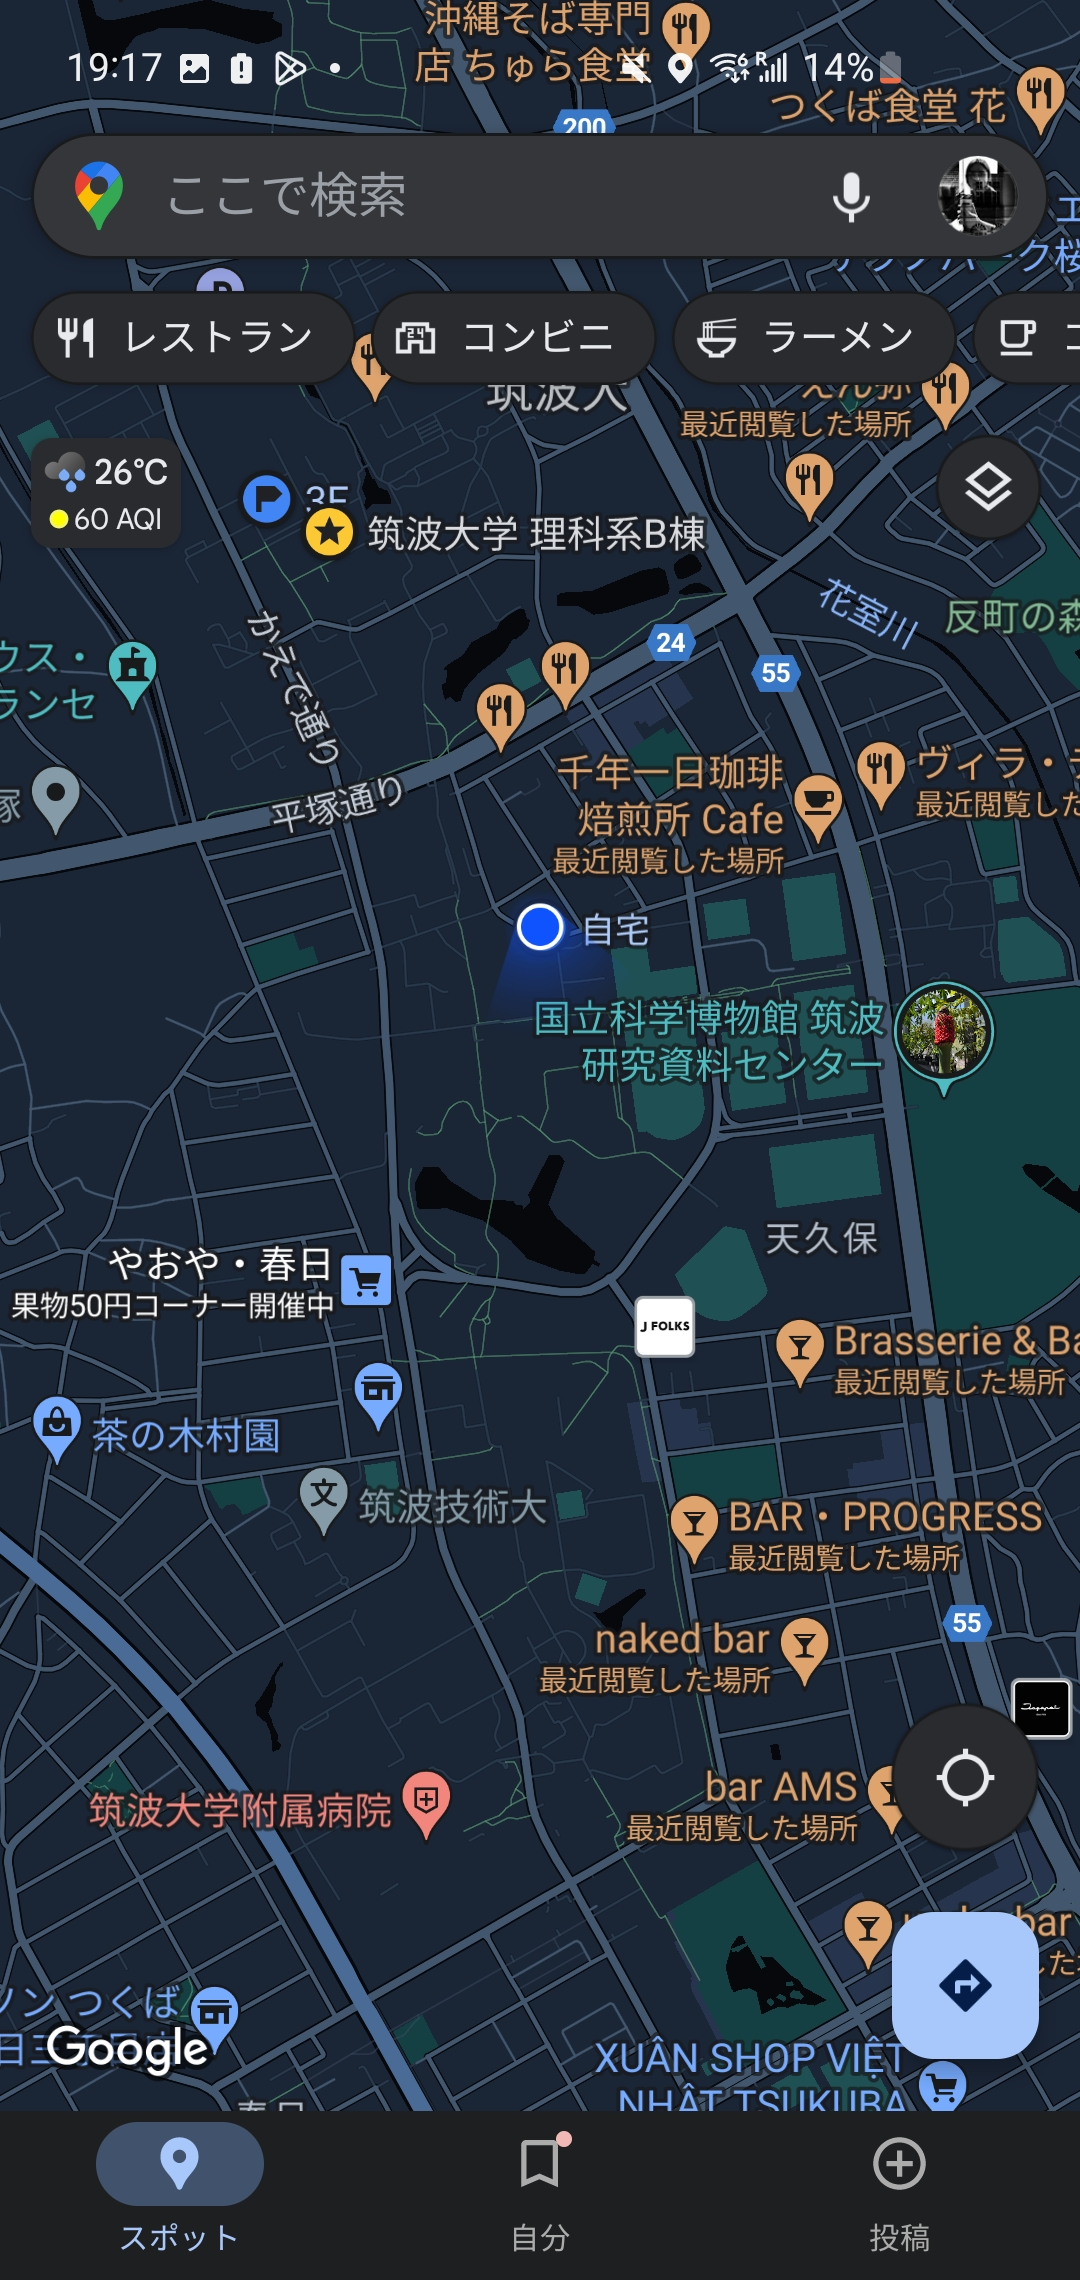
\includegraphics[width=0.5\textwidth]{materials/Maps1.jpg}

\newpage

\subsection{Bad Example}

\textbf{Grouped Network of Web-Systems:} University of Tsukuba official page, those related to the “Unified Authentication System”, etc.
\vspace{0.25cm} \\
\textbf{Purpose:} Providing information and services to those concerned and related to the university.
\vspace{0.25cm} \\
\textbf{Intended Users:} People related to the University of Tsukuba.
\vspace{0.25cm} \\
\textbf{Good Points (fair advantages):}
\begin{itemize}
    \item Does not overload CPU
    \item Some functions implement communication with possible feedback
    \item Manaba provides one-click “add to Google Calendar” feature
\end{itemize}
\textbf{Bad Points (desperately dire):}
\begin{itemize}
    \item Extremely confusing navigation and relation of web-pages
    \item Some functions are not working properly or do not work at all
    \item Cluttered interface with no consistency (different subdomains have completely different designs)
    \item Parts of the interface might overlap when used from a mobile device
    \item No history of search
    \item Poor labeling
    \item Some parts assume knowledge of Japanese
    \item Exceptionally slow authentication and response time from abroad
    \item Lack of FAQ
\end{itemize}
\textbf{Golden Rules:} Virtual disregard.
\vspace{0.25cm} \\
\textbf{Improvements:}
\begin{itemize}
    \item Standardize the interface
    \item Standardize web-page relations
    \item Strive for consistency and simplicity
    \item Unify twins, manaba, and kdb while refactoring methods to use their features
    \item Improve labeling
    \item Add full support for multiple languages
    \item Enhance response time
    \item Add help options
\end{itemize}

\textbf{Example screenshot:} \\ 
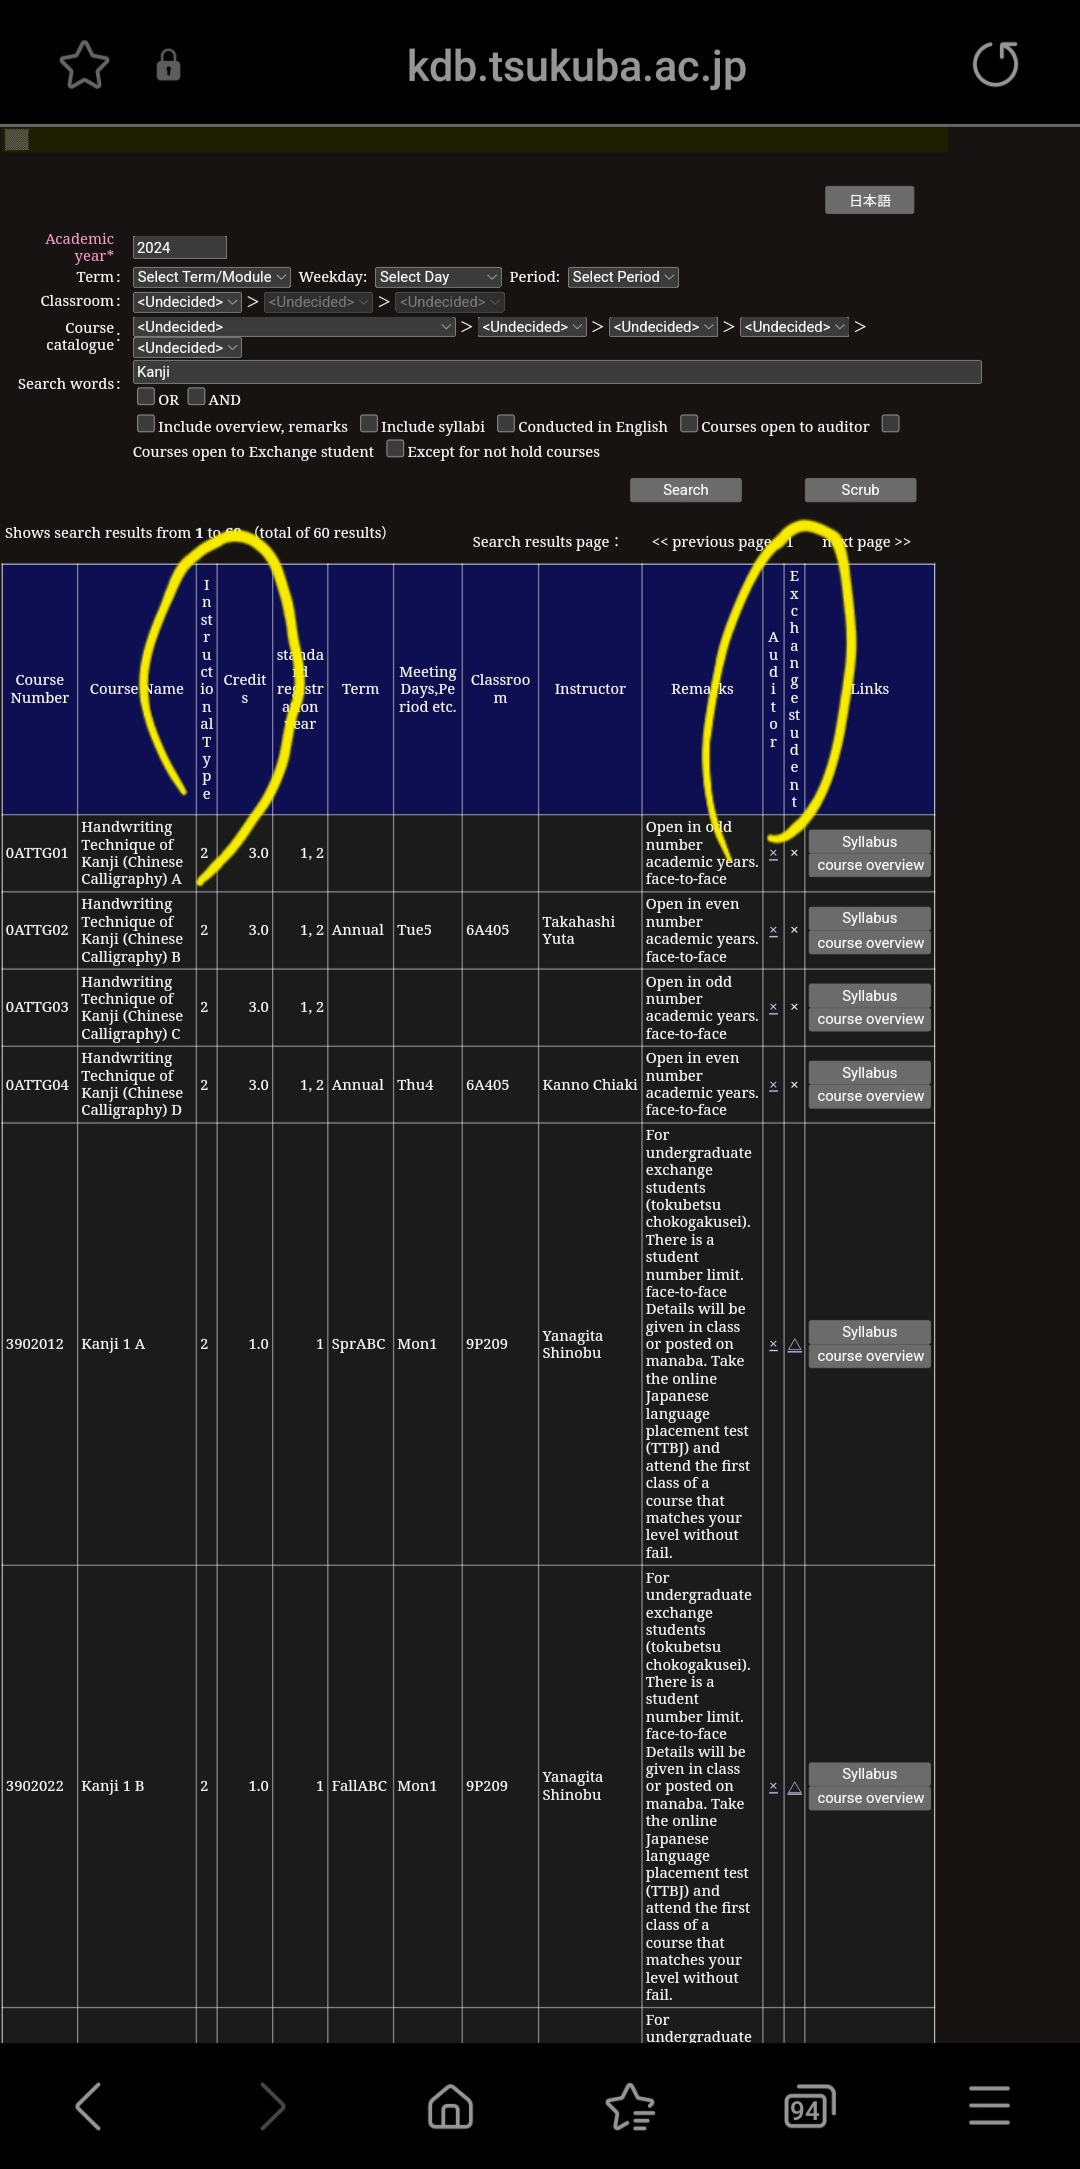
\includegraphics[width=0.5\textwidth]{materials/KDB1.jpg}

\section{Question 3 - on Agile Development}

\subsection{Good Points}
\begin{itemize}
    \item \textbf{Quite flexible to changes:} Using this methodology may imply a rapid development of the project with even integral parts able to be considered through the ongoing process of development. Secondary features or parts may be easily reconsidered, replaced, or removed.
    \item \textbf{Continuous delivery and feedback:} This suggests better handling of unexpected situations or secondary failures in the development process.
    \item \textbf{Generally quicker pace of development:} Thus, faster delivery of the final product to the market.
    \item \textbf{Improved collaboration and communication:} Essential for novice products with fresh ideas.
\end{itemize}

\subsection{Bad Points}
\begin{itemize}
    \item \textbf{Can be chaotic without proper management:} Leading to undesirable results.
    \item \textbf{May not suit all project types:} Especially those requiring a fixed scope, particularly detailed planning, or any strict approaches.
    \item \textbf{Fragmented output of development:} May not be suitable for large and complex projects.
\end{itemize}

\subsection{Unsuitable Application}
Critical infrastructure systems like medical software where extensive upfront planning and validation are required.


\section{Question 4 - on Verification and Validation}

Verification and validation are two essential processes in software development, each serving a distinct purpose to ensure the quality and suitability of the product.

\subsection{Verification}
Verification is the internal process (inside the developing organization) of ensuring that the product is built correctly according to the given requirements and specifications. It involves activities such as reviews, inspections, etc to ensure that the product meets the specified design/technical requirements. The main goal of verification is to confirm that the product development process adheres to predefined standards and methodologies.

We can define some essentials related to this process below:

\begin{itemize}
    \item \textbf{Does the product meet given requirements or not?}
    \item \textbf{Internal Quality control process - executed by a designated department}
    \item \textbf{Does not consider whether a product is suitable for customer needs}
\end{itemize}

\subsection{Validation}
Validation, on the other hand, is the process of ensuring that the product meets the customer's needs and expectations. It is an external process performed by the customer or end user. Validation involves activities such as user acceptance testing (UAT), beta/field testing to ensure that the product is fit for its intended use from the perspective of the user.

Essentials are included below:

\begin{itemize}
    \item \textbf{Does the product meet customer needs or not?}
    \item \textbf{External Scope Validation process - typically done by the customer}
    \item \textbf{Considers customer needs}
\end{itemize}

\subsection{Validation Testing: Who Should Perform It?}
In my opinion, validation testing should be performed by the end users. Since end users are the primary target audience for the software, it is crucial for them to perform validation testing before the final release. This ensures that the functionality, interface, features, usability, and overall user experience meet their expectations and are efficient from a practical standpoint.

Developers, while knowledgeable about the technical aspects of the software, may have a biased perspective that focuses more on the implementation details rather than the practical use of the product. End users, on the other hand, can provide valuable insights into the software's usability and suggest additional features or improvements, such as shortcuts for frequent actions, which may be closely related to the specific application domain.

Therefore, a comprehensive validation process should involve both developers and end users. Initially, developers can perform preliminary validation to ensure that the product is functional and free of major defects. Subsequently, end users should conduct thorough validation testing, supported by manuals or suggestions from developers, to evaluate the software's usability and overall user experience. This dual approach ensures that the software is both technically sound and user-friendly.

\section{Question 5 - on Project Managers as Robots}

The prospect of robot project managers offers potential efficiencies in handling data-intensive aspects of our conventional project management process. These robots, can be powered by AI, thus leverage advanced decision-making algorithms and data analysis to optimize project scheduling, resource allocation, risk management, etc regardless of an experience in a particular sphere, which is desirable for a managing person.

\subsection{Key Programming Aspects}

I wouldn't really imagine a particular efficient approach to program robots which are to succeed in project management solely. Albeit, to ensure effectiveness of such assistants, we would need to focus on implementing the following features and capabilities:
\begin{itemize}
	\item \textbf{Advanced AI for Decision-Making:} Utilize machine learning to refine algorithms based on project outcomes, enhancing predictive accuracy and decision quality.
	\item \textbf{Team Management Support:} While robots can oversee logistical tasks, human-like interaction remains essential for managing complex team dynamics and fostering collaboration.
	\item \textbf{Adaptability:} Projects are dynamic; thus, robots must quickly adapt plans based on real-time data, mirroring the flexibility required of human managers.
\end{itemize}

\subsection{Emotional Intelligence and Human Interaction}

Despite AI's capabilities, the emotional intelligence and creative problem-solving inherent to good project managers are yet challenging to replicate in robots. These human elements are critical for motivation, stakeholder management, and navigating organizational cultures - are still best handled by humans.

At present, a good project manager excels in strategic thinking, organizational skills, and adaptability, while ensuring alignment with business goals. Such person is also distinguished by communication abilities and emotional intelligence, seeking to build strong relationships and motivate teams. The integral part of soft skills in combination with technical knowledge allows to anticipate challenges, adapt strategies, and lead projects to successful completion - something machines are still far from being successful at.

Therefore, a hybrid model where robots manage routine tasks and humans focus on strategic and interpersonal aspects could be the optimal solution. Hence, the integration of human project managers remains crucial for dealing with the nuanced aspects of project leadership.

\section{Question 6 - on Use of AI in Education}

AI is on its way to becoming an integral part of education strategies. The conventional approach, similarly at present, has been utilized for centuries, as we can refer to the following picture:
 
\begin{center} 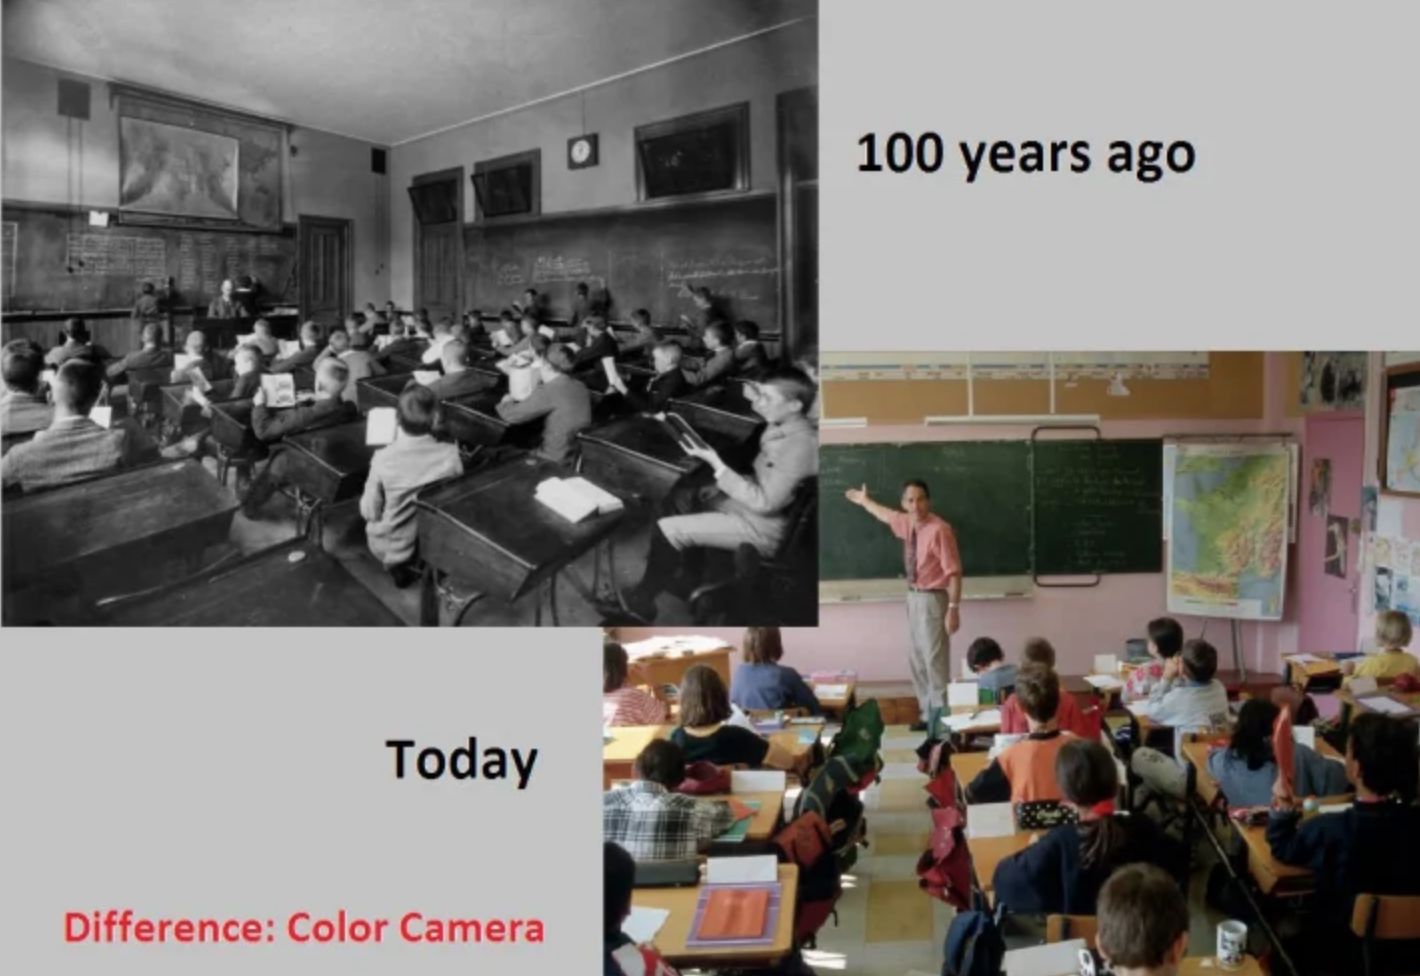
\includegraphics[width=0.5\textwidth]{materials/Classroom.png} \end{center}

There was practically no change. Nowadays, students tend to be distracted by gadgets even more, underlying whether it is a good thing to promote electronic devices during lectures. Those most diligent tend to type during the study sessions since it offers many advantages. Others can check lectures on their devices to follow up, yet conceptually everything stays the same - a teacher with maybe a couple of assistants, typically other students who help others grasp the material. 

Furthermore, the recent popularization of LLMs for surprisingly precise text generation, as I have confirmed myself, can be an extremely powerful time-saver and personal study assistant in many areas - from learning the language to fathoming advanced calculus. For those who can quickly think and incorporate complex and complete ideas in the form of text, LLMs can be even more useful yet up to a particular limit of comprehensiveness.  Ironically, while GPT and friends help with text generation, I have noticed an increase in personal typing speed since my requests frequently exceed those of GPT's neat and structured answers. Nowadays, I typically use GPT-4 for refactoring my ideas, summarizing, suggesting a set of approaches, and doing all hard work related to finding suitable commands in the terminal, googling correct syntax, or making neat files like this one using latex. In this regard, my performance has drastically increased.

From the perspective of a teacher, current implementations include AI-driven course creation, differentiated learning paths tailored to individual student needs, and automated grading systems that save time and reduce bias. These tools enhance teaching efficiency and support personalized education, enabling a shift from a one-size-fits-all approach to education that recognizes and responds to the diverse needs and pacing of individual students.

In stark contrast to the aforementioned, the use of AI can also be an insidious cheating machine. Instead of trying to understand calculus techniques - simply write it out; instead of writing an essay yourself - copy it from GPT with minor corrections - something that would be hardly detectable either by a human or by a machine. 

Despite all the negative consequences, I truly believe in the revolution of education using artificial intelligence. The impact of LLMs on the true comprehension ability of students or post-graduates is still way understudied, especially for those who use it wisely and prefer a diligent approach to their tasks. This, however, should not limit the vision of potential AI applications for students. I am not discussing the teaching perspective since I am not an experienced teacher myself and did not face those challenges. Presently, LLMs are already tuned for specific tasks. In the future, text interfaces shall, in my understanding, be replaced with all sorts of technologies, in particular, mimicking teachers themselves. This will leverage the next set of advantages:

\begin{itemize}
    \item Every student shall get a free teaching assistant with no knowledge limits;
    \item Bias in education approach corresponding to different experiences of teachers shall vanish;
    \item A unique education approach can be applied to every student based on various assessments, performance, factors, and preferences of a student.
    \item Marks can be defined based on diligence - performance is used to access strength, hence desirable areas to focus on for further development and future career, etc. Students, thus, will be naturally and gradually guided into their future life.
\end{itemize}

Underlying the discussion, I strongly believe once such an approach is realized, it may lead to outstanding results making a revolution in education methodologies.

\section{Question 7 - on Prospects of Software E/D}

\subsection{Software Development}
The integration of AI-assisted coding will significantly enhance developer performance and contribute to cleaner codebases. Traditional refactoring roles are expected to evolve into quality supervision tasks, focusing on the ethics and security of software applications. This reflects a broader industry trend towards prioritizing not just functional efficiency, but also ethical considerations and data security in software development.

\subsection{Programmers}
The role of programmers is likely to shift more towards design and oversight of AI systems rather than traditional coding. As AI improves, especially in areas like code generation and system design, human programmers will increasingly manage and refine the outputs of AI, focusing on higher-level problem-solving and system optimization tasks.

\subsection{Major Changes}
We will see greater 'collaboration' between developers and AI in software development. This will drive the creation of more sophisticated tools that integrate AI capabilities to enhance the development process, offering, for example, real-time analytics and decision support. Continuous learning and adaptation will become crucial as the landscape of software engineering evolves rapidly, requiring developers to stay current with new technologies and methodologies.

\subsection{Impact of Emerging Trends}
Technologies such as cloud computing, AI, blockchain, and cybersecurity are reshaping the demand for software engineering expertise. Each of these areas offers unique challenges and opportunities, suggesting a future where software engineers must be even more versatile, continually updating their skills to navigate a landscape of newly-emerged principles. Such a shift will require a blend of technical prowess and ethical awareness, accompanied by a strong emphasis on lifelong learning and adaptability to new technological paradigms.

% \subsection*{Listing .java}
% \begin{lstlisting}

% \end{lstlisting}

\section*{References}
\begin{enumerate}
    \item \textbf{Mamanchuk N., University of Tsukuba}, Github, \today. Available online: \url{https://github.com/RIFLE}
\end{enumerate}

\end{document}
